


\labday{Chapter 8: Shell}

\experiment{Process}
The first thing to understand is that a {\bf computer program} is a passive collection of instructions; a {\bf process} is the actual execution of those instructions.\\

A {\bf process} in user mode is not allowed to execute privileged instructions.  The only way for the process to change from user mode to kernel mode is via an exception such as an {\bf interrupt}, a {\bf fault} or a {\bf trapping system call}.


Processes can have three states:
\begin{enumerate}
\item  {\bf Running}  The process is currently running on a CPU.
\item {\bf Ready} Process could make progress if CPU were available
\item  {\bf Blocked} Process is waiting for something (memory, signal, time, etc)
\end{enumerate}


%-----------------------------------------

\experiment{Context switching} % Multiple experiments can be included in a single day, this allows you to segment what was done each day into separate categories

In computing, a {\bf context switch} is the process of storing and restoring the state (context) of a process so that execution can be resumed from the same point at a later time. This enables multiple processes to share a single CPU and is an essential feature of a multitasking operating system. What constitutes the context is determined by the processor and the operating system.\\

A context switch follows these 3 steps:

\begin{enumerate}
\item   saves the contents of the current process.
\item  restores the saved context of some previously preempted process
\item  passes control to this newly restored process
\end{enumerate}


\experiment{File Descriptor}

A file descriptor is an indicator for a way of accessing a file.


\experiment{Signal}
A {\bf signal} is a message that notifies a process that an event of some type has occured in the system (just like when you press a button on your phone, a message is sent to the operating system).  Each signal corresponds to some kind of system event.  For example, a signal can be used to cancel background jobs.\\


A pending signal is a signal that has been sent but not recieved.  A process can also block a CERTAIN signal.  In this case, blocked sigals can be sent
but will not be received until the signal is unblocked.


\begin{figure}[H] % Example of including images
\begin{center}
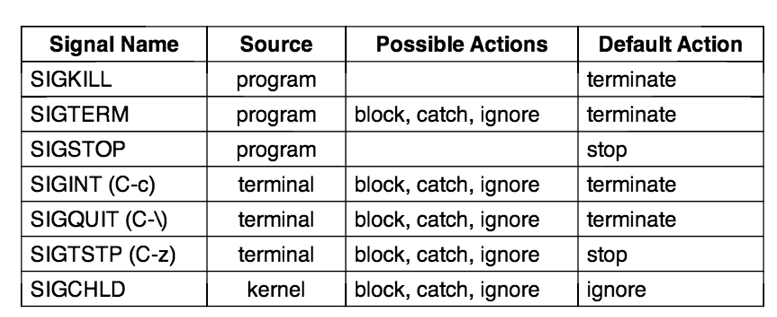
\includegraphics[width=0.5\linewidth]{signals}
\end{center}
\caption{Table of possible signals}
\label{fig:example_figure}
\end{figure}



\experiment{Pipelining}

Pipelining works by setting the standard output(1) of the first command to the standard input(0) of the second command in the pipeline.  
here are a couple of system calls that you may be interested to understand what is happening in more detail, in particular, fork(2), 
execve(2), pipe(2), dup2(2), read(2) and write(2).

\begin{itemize}
\item The dup2 function takes two parameters $dup2(old, new)$  The pointer of old will replace the pointer of new when the function is called. (code example below)
\end{itemize}

\begin{table}[H]
\begin{tabular}{l l l}
\toprule
\textbf{Integer Value} & \textbf{Name}  \\
\toprule
0 & Standard Input (Stdin)\\
1 & Standard Output (Stdout) \\
2 & Standard Error (Stderr) \\
\bottomrule
\end{tabular}
\caption{Integer Values and their File descriptors}
\label{tab:treatments_xy}
\end{table}


\newpage

\begin{lstlisting}
1	#include <stdio.h>
2	#include <unistd.h>
3	#include <sys/types.h>
4	
5	#define IN 0
6	#define OUT 1
7	
8	int main(void)
9	{
10	  char string[] = "Hello, world!\n";
11	  char readbuffer[80];
12	
13	  // Creates the pipe using the integer array of size two.
14	  int fd[2];
15	  pipe(fd);
16	
17	  // Fork new process
18	  if(fork() == 0)
19	  {
20	    // Copy the write end of pipe to standard out.
21	    dup2( fd[OUT], OUT );
22	    // Close read and write end of pipe.
23	    close( fd[IN] );
24	    close( fd[OUT] );
25	    // Child Process: execute new process
26	    char *cmd[] = {"ls", "-la", (char *) 0};
27	    execvp("ls", cmd);
28	  }
29	  else
30	  {
31	    // Clise write end of pipe.
32	    close( fd[OUT] );
33	    // Parent Process: Read string from the read side of pipe.
34	    read( fd[IN], readbuffer, sizeof(readbuffer) );
35	    printf("Received string: %s", readbuffer);
36	  }
37	  return(0);
38	}
\end{lstlisting}

 \newpage
\experiment{Fork}

This is an example of the fork method in C.  fork() clones a process from a process.  This new process can be used to execute another process or
do other things.  NOTE:  Once you clone a process you have no idea which order your clones will run in, your code should not depend on the order.  Another thing to remember is that fork returns twice, once in the parent and once in the child (the new process you just created).  The cloned process is exactly the same except for the return value of fork().  In the child process fork will always return 0 and in the parent it will return the process ID of itself so your code can just check for the child process with == 0 and the parent with an else.\\

Fork returns the PROCESS ID OF ITS CHILD to the parent process, so that the parent knows its PID of the child to keep track of it.  Fork() returns 0 to the child, you don't need it.
\begin{lstlisting}
#include <unistd.h>
#include <stdio.h>

int main(){
	int x = 1;
	
	int pid = fork();// pid contains the childs pid for the parent process.
	if (pid== 0) 
	{// only child executes this
		printf("Child, x = %d\n", ++x);
	} 
	else {
	// only parent executes this
		printf("Parent, x = %d\n", --x);
	}// parent and child execute this
	printf("Exiting with x = %d\n", x);
	return 0;
}
\end{lstlisting}

\experiment{reentrant}


A computer program in {\bf reentrant} if it can be interrupted in the middle of its execution and then safely called again.  An interuption can come from a signal or a jump.  Once the reentered invocation completes, the previous invocations will resume correct execution.

\begin{itemize}
\item Printf() is a NON reentrant function, meaning that it is not safe to interrupt.
\end{itemize}

\experiment{Signal Handlers}
Signal handlers are used to deal with the different types of signals on a USER LEVEL.\\

When a handler function is invoked on a signal, that signal is automatically blocked (in addition to any other signals that are already in the process's signal mask) during the time the handler is running. \\




\experiment{PID-process identifier}
A number used to temporarily uniquely identify a process.\\
One may use the command "ps j" to see PPID (parent process ID), PID (process ID), PGID (process group ID) and SID (session ID) of processes.   \\

Every process can have a PID, parent ID, and a group ID(gid).  A group ID means that all of the processes share the terminal together and you do not need to transfer control for these processes.  When you send a signal to a terminal, everything in the terminal control group (same gid) will receive that signal. When you send a signal via kill(), it depends on how you structure the arguments.
